{\bf Task~1.}~~{\it Read the following text. Translate the unslerlined words into Russian using the
vocabulary given in the end of the book.}\par
Within customer premises the importance of the cabling infrastracture is similar to that of other
fundamental building utilities such as heating, lighting and mains power. As with other utilities,
interruptions to service can have serious impact. Poor quality of service due to lack of design foresight,
use of inappropriate components, incorrect installation, poor administration or inadequate support can
threaten an organization's effectiveness.\par
Historically, the cabling within a premises comprised both application specific and multipurpose
networks. Appropriate use of the International Standard will enable a controlled migration to generic
cabling. Certain circumstances may warrant the introduction of application specific cabling; these
instances should be minimized.\par

{\bf Task~2.}~~{\it Read the text given in {\bf task 1} again and translate the following words and word
combinations into Russian.}\par
Fundamental, must impuct, interruptions to service, serious impact, poor quality, luck, design
foresight, inappropriate, components, controlled migration, circumstances, warrant, introduction, instances.\par

{\bf Task~3.}~~{\it Retell the text from {\bf task 1}.}\par

{\bf Task~4.}~~{\it Translate the following word combinations into Russian. Use the vocabulary given in the end
of the book}\par
Application independent generic cabling system; open market for cabling components; flexible
cabling scheme; building professionals; accomodution \textbf{FFF} of cabling; initial planning; refurbishment;
stundardisation bodies; current product; product development; multi-vendor cabling; ropper cabling;
premises geography; general pffice environment; life expectancy.\par

{\bf Task~5.}~~{\it Translate the following sentences into English.}\par
\begin{enumerate}
    \item {Структурированная кабельная система используется в коммерческих помещениях,
    расположенных в отдельных зданиях или группах зданий одного комплекса.}
    \item {Данная структурированная кабельная система предназначена для огромных помещений площадью 1000000 м$^2$.}
    \item {Кабельная система, определенная данным Международным стандартом, поддерживает
    широкий диапазон услуг, включая голосовые, видео, передачу изображения, текста и данных.}
    \item {Необходимо определить структуру и минимальную конфигурацию кабельной системы, а
    также требования к работе определенных кабельных соединений}
    \item {При установке и монтаже кабельной системы необходимо учесть требования 
    противопожарной безопасности}
    \item {В данном стандарте предлагается следующее определение кабельного элемента:
    кабельный элемент -- наименьшая составляющая кабеля; кабельный элемент может быть защищен.}
    \item {Конфигурация кабельной системы должна соответствовать требованиям, изложенным в
    разделе 5}
    \item {Вся кабельная система состоит из соединений, уровень которых соответствует стандарту}
    \item {Во многих сериях интерфейс сети общего пользователя является точкой соединения
    оборудования провайдера сети и кабельной системы помещений пользователя.}
\end{enumerate}

{\bf Task~6.}~~{\it Read the following terms. Translate them into Russian. Try to give their definition in
English.}\par
Application, balanced cable, building backbone cable, buildiny distrubutor, buildiny entrance
facility, cable unit, campus backbone cable, campus distributor, channel, cross-connect, equipment cable,
equipment room, floor distributor, horizontal cable, hybrid cable, individual work area,
interconnect, jumper, keying, optical fibre cable, optical fibre puplex adapter, patch cord, patch panel.\par

{\bf Task~7.}~~{\it Read the following definitions. Find the corresponding terms from the ones given in the frame \par}
\begin{framed}
    Work area cable; permanent link; transition point; twisted pair; telecommunications outlet;
    shielded twisted pair cables; public network interface; telecommunications closet; unshielded
    twisted pair cable; splice; work area; telecommunications; star quad.
\end{framed}
location in the horizontal cabling where a change of cable form takes place; for example flat cable
connects to round cable or cables with deffering numbers of elements are joined;\\
a cable element which consists of two insulated conductors twisted together in a regular fashion to
form a balanced transmission line;\\
an electricallu conducting cable comprising one or more pairs none of which is shielded. There may
be an overall shield, in which case the cable is referred to as unshielded twisted pair with an overall shield;\\
a building space where the occupants interact with telecommunications terminal equipment;\\
a cable connecting the telecommunications outlet to the terminal equipment;\\
the transmission path between two mated interfaces of generic cabling, excluding equipment cables,
work area cables and cross-connections;\\
a point of demarcation between public and private network. In many cases the public network
interface is the point of connection between the network provider's facilities and the customer premises
cabling;\\
an electrically conducting cable comprising one or more elements, each of which is individually
shielded. There may be an overall shield, in which case the cable is reffered to as a shielded twisted
pair cable with an overall shield;\\
a joining of conductors and fibres, generally from separate sheaths;\\
a cable element which comprises four insulated conductors twisted together. Two diametrically
facing conductors form a transmission pair;\\
a branch of technology concerned with the transmission, emission and reception of signs, signals,
writing, images and sounds; that is, information of any nature by cable, radio, optical or other
electromagnetic systems. The term telecommunications has no legal meaning when used in this
International Standard;\\
an enclosed space for housing telecommunications equipment, cable terminations, and cross-connect cabling.
The telecommunications closet is a recognized cross-connect point between the backbone and horizontal
cabling subsystems;\\
a fixed connecting device where the horizontal cable terminates. The telecommunications outlet
provides the interface to the work area cabling.\par

{\bf Task~8.}~~{\it Read the text below and answer the following questions: \par}

\begin{enumerate}
    \item How many subsystems does generic cabling contain?
    \item What do distributors provide?
    \item What does the campus backbone cabling subsystem include?
    \item Where does the building backbone cabling subsystem include?
    \item How should all cabling elements at the FT be terminated?
    \item What does the work area cabling do?
    \item What assumptions have been made?
    \item What is a general cabling?
    \item What does the number and type of subsystems depend upon?
\end{enumerate}
\par
The horizontal cabling subsystem extends from FD(s) to the TO(s). The subsystem includes the
horizontal cables, the mechanical termination of the horizontal cables at the FD, the cross-connections
at the FD and the TOs\par
Horizontal cables should be continuous from the FD to the TOs. If necessary, one TP is permitted
between an FD and any TO. The transmission charachteristics of the horizontal cabling shall be
maintained. The incoming and outgoing pairs and fibres at the TP shall be connected so that a 1:1
correspondence is maintained. All cable elements at the TP shall be mechanically terminatrd. The TP
shall not be used as a point of administration (that is, not used as a cross-connect), and application
specific equipment shall not be located there. The TP may only contain passive connecting hardware.\par
The work area cabling connects the TO to the terminal equipment. It is non-permanent and
application specific and therefore lies outside the scope of this International Standard. Assumptions
have been made concerning the length and the transmission performance of the work area cable; these
assumptions are identified when relevant.\par
The generic cabling is a hierarchial star structure which may take the form shown in figure \ref{interrelationship}. The
number and type of subsystems that are included in generic cabling implementation depnds upon the geography and size of
the campus or building, and upon the strategy of the user. For example, in a campus having only one building the 
primary distribution point is the BD, and there is no need for a campus backbone cabling subsystem. On the other hand,
one large building may be treated as a campus, with a campus backbone subsystem and several BDs. Further information on
the application of the cabling structure is given in the \textbf{JJJ}.
\begin{figure}[h]
    \centering
    \begin{framed}
         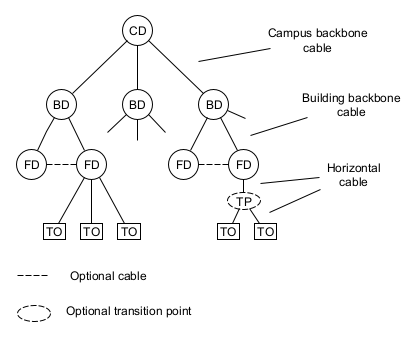
\includegraphics[height=0.3\textheight]{pics/interrelationship}
        \caption{interrelationship of functional elements}
        \label{interrelationship}
    \end{framed}
\end{figure}

Cables shall be installed between adjacent levels in the structure. This forms a hierarchial star as shown in figure 
\ref{interrelationship}, and provides the high degree of flexibility needed to accomodate a variety of applications. Annex
D details how to configure various networks within the boundaries of the hierarchial star topology. These topologies are
established by the interconnection of the cable elements at cross-connects, and at the application specific equipment.\par

For some applications, additional direct connections between FDs or DBs are desirable and are permitted. The building
backbone cable may also interconnect FDs. However, such connections shall be in addition to those required for the basic
hierarchial ster topology.\par

{\bf Task~9.}~~{\it Read the text 8 again and find the English equivalents of the following sentences: \par}

\begin{enumerate}
    \item {Распределительные пункты обеспечивают конфигурацию кабельной системы для поддержки различных топологий,
    таких как шина, звезда и кольцо}.
    \item {Подсистема магистрального кабеля в комплексе зданий проходит от СД к ВД, обычно расположенным в отдельных
    зданиях}.
    \item {Расположенные в зданиях магистральные кабели не должны содержать ТР; медные магистральные кабели не должны
    иметь сплайсов}.
    \item {Кабельная система рабочей области соединяет ТО с терминальным оборудованием}.
    \item {Количество и тип подсистем, входящих в структурированную кабульную систему, зависит от географии и размера
    комплекса зданий или отдельного здания, а также от стратегии пользователя}.
\end{enumerate}

{\bf Task~10.}~~{\it Write out all the terms from text 8, translate them into Russian, make up 10 sentences with
these terms. \par}

{\bf Task~11.}~~{\it Think over a title for text 8. Retell the text. \par}

{\bf Task~12.}~~{\it Read the text and find the sentences the beginnings of which are given below. Translate them into
Russian \par}

\begin{itemize}
    \item The design of general \dots
    \item A minimum of one TO \dots
    \item When a TO is \dots
    \item Emerging belanced cable \dots
\end{itemize}

\begin{center}
    \textbf{Telecommunications outlets}\par\par
\end{center}

TOs are located on the wall, floor, or elsewhere in the work area, depending on the design of the building. The design of 
generic cabling should provide for TOs to be installed in readily accessible locations throughout the usable floor space.\par

A high density of TOs will enhace the flexibility of the cabling to accomodate changes. In many countries two TOs are
provided to serve a maximum of $10m^2$ of usable floor space.\par

TOs may be presented singly, pr in groups, but each work area shall be served by a minimum of two.\par

A minimum of one TO served by 100 $\Omega$ or 120 $\Omega$ cable shall be provided at each work area (100 $\Omega$ preferred).
Other TOs shall be supported by either balanced cable or by fibre optical cable. In the horizontal cabling, at least one
TO shall be configured as specified in item b of balanced or optical fibre cable or at least one TO shall be served by 
either class D or optical class. When a TO is supported by balanced cable, 2 pairs or 4 pairs shall be provided at each TO;
all pairs shall be terminated. If less than four pairs are provided, the outlet shall be clearly marked. Emerging balanced
cable applications may be limited by differential delay of pairs that serve a single telecommunications outlet.\par

{\bf Task~13.}~~{\it Ask 5 questions to the text from task 12. Retell the text. \par}

{\bf Task~14.}~~{\it Compose sentences of your own with the following words and word combinations from text 12: \par}

Telecommunications outle, serve, balanced cable, generic cabling, design, horizontal cabling, floor space, application,
optical fibre cable.\par

{\bf Task~15.}~~{\it Read the following words and word combinations and translate them into Russian: \par}

Telecommunications closet, equipment rooms, earthing, entrance facilities, bonding,
electromagnetic capability, passive components, local regulations, pathway, private network,
premises cabling, backbone cabling subsystem, cable length, point of termination, balanced cable,
cabling link, performing component, mechanical termination, total length, differing requirements,
maximum cable length, work area cable, interconnect floor distributor, crossconnect, performance
charachteristics, patch cords, flexible cable, transition point, inclusion, hierarchial level, individual
cable, entire distance. hierarchial star, signal degradation, keep track of cables, entire distance,
hybrid cable, multiunit cable, accomodating ring.\par

{\bf Task~16.}~~{\it Read the text given below. Translate it into Russian. Then ask your neighbour to
translate it from Russian into English sentence after sentence. \par}

There shall be no more then two hierarchial levels of cross-connects in the backbone
cabling to limit signal degradation for passive systems and to simplify administration in keeping
track of cables are connections. No more than one cross-connect shall be passed through to reach
the CD when starting from a FD. \par

A single backbone cabling cross-connect may meet the cross-connect needs of the entire
backbone subsystem. Backbone cabling cross-connects may be located in telecommunications
closets or equipment rooms. See annex D for guidance on accomodating ring, bus, tree, etc.
configurations within the hierarchial star.\par

The star topology is applicable to the cable elements of the transmission medium, such as
individual fibres or pairs. Depending on the physical charachteristics of a site, cable elements that
are terminated at different locations may be part of the same cable over a portion of the distance, or
may use individual cables over the entire distance. Hybrid and multi-unit cables that meet the 
requirements of 8.3 may be used in the backbone cabling subsystem.\par

{\bf Task~17.}~~{\it Read the following text and together with your neighbour, compose a dialogue on its basis. \par}

The performance of a permanent link is specified at and between interfaces to the link. The
permanent link comprises only passive sections of cable and connecting hardware. A transition
point may also be included in the horizontal subsystem. Active and passive application specific
hardware is not addressed by the International Standard.\par

The optical fibre and balanced cable links are connected together using an optical fibre to
balanced cable converter, a cross-connect and two equipment cables. Interfaces to the cabling are at
each end of a permanent link. Interfaces to the cabling are specified at the TO and at any point
where application specific equipment is connected to the cabling; the work area and equipment
cables are not included in the permanent link.\par

Interfaces to the cabling are at each end of a permanent link. Interfaces to the cabling are
specified at the TO and at any point where application specific equipment is connected to the
cabling; the work area and equipment cables are not included in the permanent link.\par

The performance of the channel is specified at and between interfaces to the channel. The
cabling comprises only passive sections of cable connecting hardware, work area cords, equipment
cords and patch cords.\par

The optical fibre and balanced cabling channels are connected together using an optical fibre to
balanced cable converter. There are four channel interfaces; one at each end of the copper channel,
and one at each end of the optical fibre channel. Equipment connections are not considered to be
part of the channel. All work area, equipment cables and patch cords are included in the channel.\par

Consideration should be given, when specifying and designing cabling, to the possible future
connection of cabling subsystems to form longer links and channels. The performance of these
longer links and channels will be lower than that of any of the individual subsystem links and
channels from which they are constructed. Measurement of permanent links and channels should be
made, initially, upon installation of each cabling subsystem. Testing of combined subsystems
should be performed as required by the application.\par

{\bf Task~18.}~~{\it Read the following sentences. Put them in the right order to make a text.
Read this text and retell it. \par}

\begin{enumerate}
    \item {The performance requirements of single-mode and multimode optical fibre permanent 
    links/channels are considered in this clause.}
    \item {The performance requirements for optical fibre permanent links/channels assune that
    each optical fibre permanent link/channel employs a single optical wavelength in one
    transmission window only}.
    \item There are no special requirements for generic cabling concerning wavelength multiplexing.
    \item Application standards employing wavelength multiplexing are not yet available for listing.
    \item {The requirements for the wavelength multiplexing and demultiplexing components will
    be found in the application standards}.
    \item {All application specific hardware for wavelength multiplexing is installed in the
    equipment area and in the work area}.
\end{enumerate}

{\bf Task~19.}~~{\it Give the following a two way translation. \par}

\begin{itemize}
    \item {All cables shall meet the appliable safety requirements as specified by the relevant local
    authorities}.
    \item {Из-за ограничений некоторых услуг связи использование осписанных ниже кабелей
    для поддержки других применений не всегда дает приемлемое качество предоставляемых услуг}.
    \item {The user is advised to consult standards associated with the planned service or equipment in
    order to determine any specific limitation}.
    \item {Требования к потерям при затухании даны только для дискретных частот}.
    \item {They have to be fulfilled, however, for all intermediate frequencies}.
    \item {Требования к промежуточным частотам устанавливаются посредством линейной
    интерполяции между двумя специфическими частотами по семи -- логарифмической шкале}.
    \item {For multimode and single-mode fibre a conservative conversion value for unit propagation
    delay of 5.00 ns/m (0.667 c) may be used}.
    \item {Эта величина может использоваться для расчета задержки в канале без проверки}.
\end{itemize}

{\bf Task~20.}~~{\it Give a summary of text 17. \par}

{\bf Task~21.}~~{\it Fill in the blanks with the words from the frame. Translate the sentences received into Russian. \par}

\begin{framed}
    Outlets; horizontal; backbone; crosstalk; connectors; category; units; transmission; optical fibre;
    network; cabling; connecting; installed cabling systems; cross-connect jumpers
\end{framed}

\begin{enumerate}
    \item In the \blank cabling subsystem cables that contain more than two pairs shall meet the requirements.
    \item {In the \blank cabling subsystem when multiple telecommunications \blank are served by a
    single cable the near-end \blank of cable elements that extend to any two or more outlets shell
    meet the requirements.}
    \item The \blank may be of the same type or of different types, and of the same \blank or of
    \item different categories.
    \item Unless otherwise specified all \blank shall be tested in a mated state.
    \item {When required such devices are not considered to be part of the \blank and may have
    significant detrimental effects on \blank performance.}
    \item {The three parts to the requirements for \blank cable are the optical fibre requirements, the
    cable \blank performance and the physical cable requirements}.
    \item The \blank hardware shall be designed to operate reliably for temperature ranging from -10C to 60C.
    \item Cables used for \blank and patch cords are subject to the performance requirements.
    \item {The manner and care with which the cabling is implemented are a significant factor in the
    performance and ease of administration of \blank}.
\end{enumerate}

{\bf Task~22.}~~{\it Read the following extracts. Put them in the right order so as to form a text. Read
the text and retell it \par}

\begin{enumerate}
    \item {Unless the network analyser is equipped with balanced outputs, baluns are required to
    provide transmission continuity to the balanced test leads. Test baluns shall be RFI (Radio
    Frequency Interference) shielded and sjall comply with the specifications listed in table}
    \begin{longtable}[c]{| p{4cm} | p{4cm} |}
        \caption{Test balun performance charachteristics (1 MHz - 100 MHz)} \\
        \hline
        {\bf Parameter} & {\bf Value} \\
        \hline
        Impedance, primary 1) & 50 .O (unbalanced) \\
        \hline
        Impedance, sec:Jnda 2) & 100 .o, 20 Q or 150 .o (balanced) \\
        \hline
        Attenuation & 1,2 dB max. \\
        \hline
        Return loss, bi-directional & 20 dB min. \\
        \hline
        Power rating & 0.1 min. \\
        \hline
        Longitudinal balance & 50 dB min. \\
        \hline
        \multicolumn{2}{|p{8cm}|}{
            1) Primary impedance may differ, if necessary to accomodate analyser outputs other than 50 $\Omega$.
            }\\
            \multicolumn{2}{|p{8cm}|}{
            2) Balanced outputs of the best baluns shall be matched to the nominal impedance of the test leads
            }\\
            \multicolumn{2}{|p{8cm}|}{
            3) Measured per ITU-T Recommendations G.117 and 0.9
            }\\
        \hline
    \end{longtable}
    \item {Balanced test leads are used for connections to and from the test sample. Test leads shall
    be taken from cables that meet or exceed requirements for the highest performance $100 \Omega$, $120 \Omega$ or
    $150 \Omega$ cable given in clause 8 or annex C}. The balanced test leads shall be limited to a length of 65
    mm between each balun and the connector under test. If used, coaxial cable assemblies extending to
    and from test equipment should be as short as possible. It is recommended that they do not exceed
    the balanced test leads at the point they are connected to the baluns. In addition, separation between
    the active conductors of the product under test and the balun ground plane (if present) shall be at
    least 50 mm. If the balanced test leads are shielded. the shield shall be connected in common with
    the balun casing on at least one end.
    \item {For pairs not under test, impedance matching terminations are not required on the near
    end. Product orientation, with respect to near-end and far-end, may affect measurement results. Due
    to these effects, the connector shall be tested in the orientation that best reflects installed field use.
    Products that are intended to receive near-end signals from either orientation (for example, those
    that may be used as TOs as well as in telecommunications closets for patching) shall be tested in
    both orientations for NEXT loss, attenuation, and return loss}.
    \item {For crosstalk measurements, near-end of the transmission test setup corresponds to the
    end from which test signals are applied. Far-end is defined as the end of the product under test that
    is not directly connected to measurement equipment. For NEXT loss and return loss measurements,
    pairs at the far-end are terminated with impedance matching terminations}.
    \item {Impedance matching terminations for the balanced test leads and the product under test
    shall be matched to the nominal impedance of the test leads (in particular $100 \Omega$, $120 \Omega$ or $150 \Omega$)
    with a tolerance not to exceed $\pm 3\%$ ($\pm 1\%$ precision metal film or precise low inductance resistors
    are recomended), throughout the Frequency range from 1 MHz to 100 MHz}.
\end{enumerate}

{\bf Task~23.}~~{\it Revise the information received in tasks 1-22. Enlarge it with your own knowledge
of cabling systems. Compose a story devoted to that subject. \par}

{\bf Task~24.}~~{\it Find in the vocabulary English terms corresponding to the following Russian definitions: \par}

\begin{itemize}
    \item {кабель, проложенный методом открытой проводки на опорах вне и между зданиями без защиты
    от воздействий внешней среды;}
    \item соединительный кабель, используемый для подключения оборудования в рабочей области;
    \item система прокладки кабелей между подвесным или фальшпотолком и структурной поверхностью над ним;
    \item цилиндрический кабелепровод;
    \item физический канал передачи сигналов между распределительными пунктами зданий;
    \item площадь этажа, которую можно использовать под офисы;
    \item среда, обеспечивающая распространение электромагнитных сигналов;
    \item проводник без разъемов для коммутации на кронах;
    \item разъем для подключения оборудования к структурированной кабельной системе;
    \item площадь помещения, отведенная пользователю.
\end{itemize}

{\bf Task~25.}~~{\it Read the following terms. Find theit Russian definitions in the vocabulary.
Translate them into English. \par}

\noindent Alien crosstalk, crossover, delay, linkage, mode, twisted pair, termination, inconduit, user code,
warranty, straight cable, splice, record, interconnect panel, horizontal cabling, identifier, fiber to the
desk, firestop, entrance facility, duct, active equipment, balanced transmission, unshielded twisted
pair, raceway, trough, plug, protocol, octopus, grounding electrode, furniture cluster, class, cabinet,
alternate entrance.
